\documentclass[times, utf8, diplomski]{fer}
\usepackage{booktabs}
\usepackage[utf8]{inputenc}

\usepackage[T1]{fontenc}
\usepackage{fixltx2e}
\usepackage{graphicx}
\usepackage{longtable}
\usepackage{float}
\usepackage{wrapfig}
\usepackage{soul}
\usepackage{textcomp}
\usepackage{marvosym}
\usepackage{wasysym}
\usepackage{latexsym}
\usepackage{amssymb}
\usepackage{hyperref}
\usepackage{caption}
\usepackage{pdfpages}
\usepackage{float}
\usepackage[usenames, dvipsnames]{color}
\usepackage{listings}
\usepackage{xcolor}
\usepackage{subfig}
\usepackage{algpseudocode}
\usepackage[Algoritam]{algorithm}

\lstset { %
    language=C++,
    backgroundcolor=\color{black!5}, % set backgroundcolor
    basicstyle=\footnotesize,% basic font setting
}


\begin{document}

\thesisnumber{570}

\title{Tool for aligning long DNA reads}

\author{Filip Paveti\'{c}}

\maketitle

% Ispis stranice s napomenom o umetanju izvornika rada. Uklonite naredbu \izvornik ako želite izbaciti tu stranicu.
\izvornik

% Dodavanje zahvale ili prazne stranice. Ako ne želite dodati zahvalu, naredbu ostavite radi prazne stranice.
\zahvala{}

\tableofcontents

\chapter{Introduction}
Uvod rada. Nakon uvoda dolaze poglavlja u kojima se obrađuje tema.

\chapter{Preliminaries}

From algorithmic point of view, aligning reads to a reference genome comes down to string pattern matching. When looked that way, one does not have to know a lot of biology background in order to understand how the existing alignment systems work. However, to understand a wider picture it is useful to know some basic genetics. 
\\
\\
This chapter is intended to give a short introduction to genetics. There exist many resources which cover this topic in far more depth\cite{griffiths}\cite{brown}. Additionaly, terminology used through rest of the Thesis is introduced. In the end of the chapter, basic alignment algorithms are discussed in details.

\section{Genetics}
\subsection{Overview}

\emph{Genetics} is a field of science which studies \emph{genes}. Genes are the carrier of biological information in the living organisms. They are responsible for inheritance of features from organisms to their offsprings. Aside from carrying that hereditary information, the role of genes inside a cell of an organism is to dictate production of molecules called \emph{proteins}. If we think of a gene as a part of the cell which commands what to do, protein is the part which does the job. Each type of protein is specialized for a particular job, such as catalyzing metabolic reactions, replicating  DNA or transporting molecules from one place to another.
\\
\\
Protein is structured as a chain of twenty different kinds of molecules called \emph{amino-acids}. Interaction between those molecules causes the protein to fold into a compact shape (Figure \ref{myoglobin}). Shape and sequence of amino-acids determine what a protein does. For example, protein can match the shape of another molecule, which would allow the protein to bind around that molecule and transport it.

\begin{figure}[!ht]
\begin{center}
	\includegraphics[width=0.7\textwidth]{../img/Myoglobin.png}
	\caption{3D structure of Myoglobin protein (http://en.wikipedia.org/wiki/Myoglobin, June 11th 2013)}\label{myoglobin}
\end{center}
\end{figure}

\subsection{From genes to proteins}

\emph{DNA (deoxyribonucleid acid)} is a long molecule which encodes genetic instructions in living organisms. That molecule consists of two interconnected chains (\emph{strands}) which are consisted of alternating sugar and phosphate groups with one of four kind of \emph{nucleobases} attached to the sugars. Nucleobases found in the DNA are: guanine, adenine, thymine and cytosine encoded using letters G, A, T and C respectively. Bases on the two strands are always paired: next to adenine on one strand there is always thymine on the other. Next to guanine there is always cytosine. Due to their chemical composition, strands have directionality. Ends of strands are denoted by 5' and 3'. Those numbers refer to the orientation of fifth and third carbon atom sugar molecules are facing. Many processes involving DNA are directed (for example, replication occurs only in 5'-3' direction). Total DNA of an organism is packed inside of one or more structures called \emph{chromosomes}. Genes are only special segments of DNA which encode instruction for protein production. Set of all genes in an organism is called the \emph{genome}.
\\

\begin{figure}[!ht]
\begin{center}
	\includegraphics[width=0.5\textwidth]{../img/DNA_chemical_structure.pdf}
	\caption{DNA chemical structure (http://en.wikipedia.org/wiki/Genes, June 11th 2013), Madeleine Price Ball}\label{dna.chemical.structure}
\end{center}
\end{figure}

Process of protein production contains several steps. First, cell reads a gene and \emph{transcribes} it into \emph{RNA} chain. That molecule either has a function on its own or is passed to a structure called \emph{ribosome} - its role is to \emph{translate} received RNA to a protein.
\\

\begin{figure}[!ht]
\begin{center}
	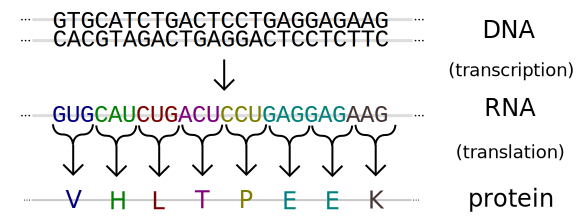
\includegraphics[width=0.7\textwidth]{../img/Genetic_code.pdf}
	\caption{DNA chemical structure (http://en.wikipedia.org/wiki/Introduction\_to\_genetics, June 11th 2013), Madeleine Price Ball}\label{genetic.code}
\end{center}
\end{figure}

Transcription step is conceptually straight forward - one of the strands of DNA is copied replacing every thymine (T) occurence with uracil (U), creating the RNA chain. Finally in the translation step RNA is passed to a ribosome. It translates consecutive triplets of bases into corresponding amino-acids resulting in a protein. 

\section{Shotgun DNA sequencing}

Modern DNA sequencing methods can read strands up to only few thousands of bases at the time. That is why \emph{shotgun} sequencing was developed. Shotgun sequencing (shotgun cloning) is a method for sequencing long DNA strands. s name is motivated by a random firing pattern of a real shotgun - a long strand is broken at random places and each piece is read with classic DNA sequencing method.


\section{Alignment algorithms}
Prodiskutirati Needleman Wunscha i Smith Watermana te staviti detaljan
opis bandede edit(levenstein) distance algoritma.
\subsection{Edit distance}

\chapter{LISA - Longest Increasing Subsequence Aligner}
\section{Overview}
\section{Index}
\section{Alignment algorithm}
\subsection{Single alignment}
\subsection{Multiple alignment}
\section{Implementation}
\section{Installation}
\section{Usage}

\chapter{Results}
\section{Yersinia Pestis}
\section{Banana}
\section{Sloth}

\chapter{Conclusion}
Zaključak.

\chapter{Appendix}
\section{Fenwick tree}

\bibliography{literatura}
\bibliographystyle{plain}

\begin{sazetak}
Sažetak na hrvatskom jeziku.

\kljucnerijeci{Ključne riječi, odvojene zarezima.}
\end{sazetak}

% TODO: Navedite naslov na engleskom jeziku.
\engtitle{Title}
\begin{abstract}
Abstract.

\keywords{Keywords.}
\end{abstract}

\end{document}
